
%\section{Propiedades de los ácidos y bases}\label{sec:propiedades-de-los-acidos-y-bases}
%
%\begin{enumerate}[label=\numberballmDarkTeal]
%    \item \negsubro{Ácidos}
%    \begin{enumerate}[label=\(\bullet\)]
%        \item Tienen sabor agrio.
%        \item Son corrosivos para la piel.
%        \item Enrojecen ciertos colorantes vegetales.
%        \item Disuelven sustancias.
%        \item Atacan a los metales desprendiendo \ch{H2}.
%        \item Pierden sus propiedades al reaccionar con bases.
%    \end{enumerate}
%    \item \negsubro{Bases}:
%    \begin{enumerate}[label=\(\bullet\)]
%        \item Tienen sabor amargo.
%        \item Suaves al tacto pero corrosivos para la piel.
%        \item Dan color azul a ciertos colorantes vegetales.
%        \item Precipitan sustancias disueltas por ácidos.
%        \item Disuelven grasas.
%        \item Pierden sus propiedades al reaccionar con ácidos.
%    \end{enumerate}
%\end{enumerate}

    \section{Teoría de Arrhenius}
    El químico sueco \negrita{Svante August Arrhenius} propuso en \num{1887} la teoría de la \negrita{disolución iónica} para las sustancias llamadas \negrita{electrolitos}.

    \caja{Los \negrita{electrolitos}, al disolverse se disocian en dos o más componentes llamados \negrita{iones} que tienen carga eléctrica positiva o negativa}.

    Previamente, Faraday había descubierto que las disoluciones acuosas de ácidos y bases conducían la electricidad por lo que pasaron a considerarse electrolitos.

    Tras este hallazgo, Arrhenius propuso:

    \begin{enumerate}[label=\numberballmDarkTeal]
        \item \negsubro{Ácidos}: compuestos eléctricamente neutros que en disolución acuosa, se disocian produciendo hidrones \footnote{\ch{H+} se le conoce como hidrón, o también como ión hidrógeno} (\ch{H+}) e iones negativos.
        \begin{reactions*}
            HA & -> H+ + A- \\
            HCl & -> H+ + Cl-\\
            H2SO4 & -> 2 H+ + SO4^{2-}\\
            CH3-COOH & -> H+ + CH3-COO-
        \end{reactions*}

        \item \negsubro{Bases}: compuestos eléctricamente neutros que en disolución acuosa, se disocian produciendo iones hidroxilo (\ch{OH-}) e iones positivos.
        \begin{reactions*}
            BOH &-> OH- + B+\\
            NaOH &-> OH- + Na+\\
            Ba(OH)2 &-> 2 OH- + Ba^{2+}\\
        \end{reactions*}
    \end{enumerate}

    \begin{center}
        \begin{definicion}[width=0.9\textwidth]{Neutralización}
            Definimos \azuln{neutralización} como la reacción entre los \azuln{ácidos} y \rojon{bases}
        \end{definicion}
    \end{center}

    Para Arrhenius, por tanto, la \negrita{neutralización} consistiría en la reacción entre hidrones y iones hidroxilo para formar agua según la reacción:
    \begin{reaction}
        H+ + OH- -> H2O
    \end{reaction}

    Según esta definición, la reacción entre un ácido y una base es siempre muy parecida independientemente del ácido y de la base usada ya que los iones que reaccionan son siempre \ch{H+} y \ch{OH-} quedando los iones positivos y negativos restantes que forman los ácidos y las bases como meros \negrita{espectadores} de la reacción.

    \begin{reaction*}
        HCl + NaOH -> {\color{blue} H+} + \color{red} Cl- + Na+ + {\color{blue} OH-} \color{black} -> \color{blue} H2O \color{black} + \color{red} NaCl
    \end{reaction*}

    \subsection{Limitaciones de la teoría de Arrhenius}

    Las principales limitaciones de esta teoría son:
    \begin{enumerate}[label=\numberballmDarkTeal]
        \item Solo lo podemos aplicar a sustancias neutras y disueltas en agua.
        \item No es capaz de explicar el comportamiento ácido y básico de todas las especies. No podía explicar el comportamiento básico del \ch{NH3} ya que en disolución no produce iones hidroxilo.
    \end{enumerate}


    \section{Teoría de Br\o{}nsted y Lowry: ácidos y bases conjugados}
    Esta teoría fue publicada en \num{1923} de manera independiente por el científico danés \negrita{Johannes Nicolaus Br\o{}nsted} y el inglés \negrita{Thomas Martin Lowry}.

    La gran diferencia de esta teoría con respecto a la publicada por Arrhenius es que ahora el comportamiento ácido y básico de las sustancias no se establecía como algo aislado sino como algo interrelacionado, es decir, un ácido para actuar como tal necesita la presencia de una base y viceversa.

    \begin{enumerate}[label=\numberballmDarkTeal]
        \item \negsubro{Ácido}: sustancia que cede hidrones (\ch{H+}) a una base.
        \item \negsubro{Base}: sustancia que capta hidrones (\ch{H\pch}) de un ácido.
    \end{enumerate}

    Con esta nueva teoría, las reacciones de neutralización se entienden como una transferencia de hidrones entre ácidos y bases en las que el ácido cede hidrones y la base los capta.

    \begin{equation*}
        \ch{!( "\textcolor{blue}{ácido}" )(\color{blue}HA) + !( "\textcolor{red}{base}" )(\color{red}B) -> \color{red}A- \color{black} + \color{blue} HB+}
    \end{equation*}

    Como la transferencia de hidrones es reversible, la reacción también puede transcurrir al revés, ahora la especie \ch{BH+} actúa como ácido cediendo hidrones y la especie \ch{A-} actúa como base, aceptando hidrones según:

    \begin{equation*}
        \ch{HA + B <- !( "\textcolor{red}{base}" )(\color{red}A-) + !( "\textcolor{blue}{ácido}" )(\color{blue} HB+ )}
    \end{equation*}

    Al ver ambas reacciones, podemos ver que las especies químicas \ch{HA} (forma ácida) y la especie \ch{A-} (forma básica) son interconvertibles mediante la ganancia o pérdida de \ch{H+}.
    Si dice, por tanto, que ambas especies forman un \azuln{par ácido-base conjugados} representándose como \ch{HA/A-}.

    Podemos decir que \ch{HA} es el ácido conjugado de la base \ch{A-} o que la especie \ch{A-} es la base conjugada del ácido \ch{HA}.

    El mismo razonamiento, pero a la inversa podemos hacer de las especies \ch{B/BH+}.

    \vspace{10mm}
    \begin{minipage}{\textwidth}
        \centering
        \OX{a1,\ch{!( "\textcolor{red}{ácido 1}" )(\color{red} HA)}} \ch{+} \OX{b2,\ch{!( "\textcolor{blue}{base 2}" )(\color{blue}B)}} \ch{<=>} \OX{b1,\ch{!( "\textcolor{red}{base 1}" )(\color{red}A-)}} \ch{+} \OX{a2,\ch{!( "\textcolor{blue}{ácido 2}" )(\color{blue}BH+ )}}
%    \redox(a1,b1)[red]{}
%    \redox(b2,a2)[blue][-1]{}
    \end{minipage}
    \vspace{10mm}

    Para el caso particular del amoniaco y el ácido clorhídrico tendríamos:

    \vspace{10mm}
    \begin{minipage}{0.8\textwidth}
        \centering
        \OX{a1,\ch{!( "\textcolor{red}{ácido 1}" )(\color{red} HCl)}} \ch{+} \OX{b2,\ch{!( "\textcolor{blue}{base 2}" )(\color{blue}NH3)}} \ch{<=>} \OX{b1,\ch{!( "\textcolor{red}{base 1}" )(\color{red}Cl-)}} \ch{+} \OX{a2,\ch{!( "\textcolor{blue}{ácido 2}" )(\color{blue}NH4+ )}}
%    \redox(a1,b1)[red]{}
%    \redox(b2,a2)[blue][-1]{}
    \end{minipage}
%\vspace{10mm}

    \subsection{Ácidos en disoluciones acuosas}\label{subsec:acidos-en-disoluciones-acuosas}

    Según la teoría de Br\o{}nsted y Lowry los ácidos reaccionarían con el agua (disolvente) actuando en este caso como base:
    \begin{gather*}
        \ch{HA + H2O <=> A- + H3O+}\separ
        \ch{HCl + H2O <=> Cl- + H3O+}\separ
        \ch{HClO4 + H2O <=> ClO4- + H3O+}\separ
        \ch{CH3COOH + H2O <=> CH3COO- + H3O+}\separ
        \ch{H2SO4 + 2 H2O <=> SO4- + 2 H3O+}
    \end{gather*}
    La teoría de Arrhenius se limitaba a especies neutras.
    Esta nueva teoría amplía el concepto especies iónicas.
    \begin{gather*}
        \ch{NH4+ + H2O <=> NH3 + H3O+}\separ
        \ch{HSO4- + H2O <=> SO4^{2-} + H3O+}\separ
        \ch{H2PO4- + H2O <=> HPO4- + H3O+}
    \end{gather*}

    \subsection{Bases en disoluciones acuosas}\label{subsec:bases-en-disoluciones-acuosas}
    Las bases según la teoría de Arrhenius siguen siendo bases en esta nueva teoría ya que estas especies producen iones hidroxilo, que es la verdadera base según la teoría del ácido-base conjugados.

    Consideremos el \ch{KOH}, que se disociará según:
    \begin{equation*}
        \ch{KOH <=> K+ + OH-}
    \end{equation*}
    Después, estos iones \ch{OH-} reaccionarán con el agua actuando en este caso el agua como ácido según la reacción.
    \begin{equation*}
        \ch{!(base 1)(OH-) + !(acido 2)(H2O) <=> !(base 2)(OH-) + !(ácido 1)(H2O)}
    \end{equation*}

    Con esta nueva teoría, podemos ampliar el concepto también a especies iónicas.
    \begin{gather*}
        \ch{NH3 + H2O <=> NH4+ + OH-}\separ
        \ch{PH3 + H2O <=> PH4+ + OH-}\separ
        \ch{HCO3- + H2O <=> H2CO3 + OH-}\separ
        \ch{CO3^{2-} + H2O <=> HCO3- + OH-}
    \end{gather*}

    \subsection{Disoluciones no acuosas}\label{subsec:disoluciones-no-acuosas}

    Esta teoría de Br\o{}nsted y Lowry permite explicar el concepto ácido-base en disolventes distintos al agua.

    Así, sustancias ácidas en disoluciones amoniacales, el amoniaco actuará como base según la reacción:

    \begin{equation*}
        \ch{HClO + NH3 <=> ClO- + NH4+}
    \end{equation*}

    Igualmente, sustancias básicas en disoluciones amoniacales, el amoniaco ahora actuará como ácido según:
    \begin{equation*}
        \ch{N^{3-} + NH3 <=> NH^{2-} + NH2-}
    \end{equation*}

    \subsection{Comportamiento anfótero}\label{subsec:comportamiento-anfotero}

    \begin{center}
        \begin{definicion}[width=0.9\textwidth]{Anfótero}
            Decimos que una especie tiene carácter \negrita{anfótero} cuando pueda comportarse como ácidos o como bases dependiendo de las sustancias con las que reaccionen.
        \end{definicion}
    \end{center}


    A las especies con carácter anfótero se les denominan \negrita{anfóteros} y no debemos confundirlo con los \negrita{anfolitos} siendo esta última una especie que puede donar y aceptar un hidrón de manera simultánea como es el caso de los aminoácidos.

    Un ejemplo de anfótero, sería el ion hidrogenosulfuro \ch{HS \mch}, es un anfótero porque puede reaccionar como:
    \begin{itemize}
        \item \negrita{Ácido}: \hspace{2mm}\ch{!(ácido 1)(HS \mch) + !(base 2)(NH3) <=> !(base 1)(S^{2-}) + !(ácido 2)(NH4+ )}.
        \item \negrita{Base}: \hspace{2mm}\ch{!(base 1)(HS \mch) + !(ácido 2)(H2O) <=> !(ácido 1)(H2S) + !(base 2)(OH\mch)}
    \end{itemize}


    \section{Teoría de Lewis}

    El norteamericano \negrita{Gilbert Newton Lewis} introdujo un nuevo concepto de ácido y de base que acabó de desarrollar en \num{1938}.

    La teoría de Lewis plantea las reacciones ácido-base de una manera mucho más general que la transferencia de hidrones y por tanto según Lewis:

    \begin{enumerate}[label=\numberballmDarkTeal]
        \item \negsubro{Ácidos}: sustancia capaz de aceptar un par de electrones y formar un enlace covalente dativo coordinado.
        \item \negsubro{Bases}: sustancia capaz de ceder un par de electrones y formar un enlace covalente dativo coordinado
    \end{enumerate}

    \begin{figure}[H]
        \centering
        % [FIGURA ORIGINAL] \includegraphics[scale=1]{images/imagesUD7EquilibrioAcidoBase/UD7_Teoria/acidoybaselewis}
        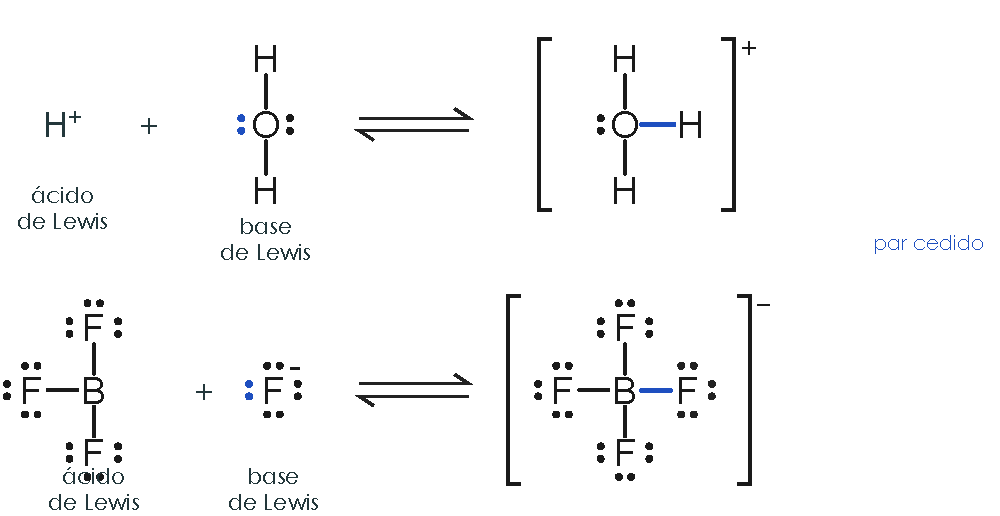
\includegraphics[width=0.7\linewidth]{FigurasSVG/UD7_Equilibrio_Acido_Base/pdf/UD7_01_acidos_bases_lewis.pdf}
        \caption{Ácidos y bases de Lewis}
        \label{fig:acidoybaselewis}
    \end{figure}

% \begin{figure}[H]
%     \centering
%     \includegraphics[scale=.7]{lewis_teoria.png}
% \end{figure}


    \section{Fortaleza de los ácidos y bases: constante de acidez y constante de basicidad}\label{sec:fortaleza-de-los-acidos-y-bases:-constante-de-acidez-y-constante-de-basicidad}

    La disociación de un ácido o una base está gobernada, como todas las reacciones por su constante de equilibrio.
    Por normal general se usa la constante de disociación o de acidez \(k_a\) para un ácido o la constante de basicidad \(k_b\) para una base donde ya está incluida la \conc{H2O} que se considera invariable.

    Sea la reacción entre un ácido general \ch{HA} y \water.

    \begin{equation*}
        \ch{!(ácido 1)(HA) + !(base 2)(H2O) <=> !(base 1)(A-) + !(ácido 2)(H3O+ )}
    \end{equation*}

    Su contante de equilibrio sería:

    \begin{gather*}
        K = \dfrac{\conc{A-}\ \conc{H3O+}}{\conc{HA}\ \conc{H2O}}\separ
        k_a = k\conc{H2O} = \dfrac{\conc{A-}\ \conc{H3O+}}{\conc{HA}}
    \end{gather*}

    A mayor valor de la constante de acidez \(k_a\) mayor será la disociación y por tanto más fuerte será el ácido.

    \begin{enumerate}[label=\numberballmDarkTeal]
        \item \negsubro{Ácidos fuertes}: están completamente disociados o casi completamente disociados en disolución diluida, es decir una concentración menor a\concentracion[m]{0.1}.
        En estos ácidos tenemos prácticamente la base conjugada (\ch{A-}) y no existen moléculas sin disociar (\ch{HA}), esto provoca que el valor de \(k_a\) sea muy alto (superior a \num{e3}) y se dice que el grado de disociación \(\bm{\alpha}\) es de prácticamente la unidad.
        En el caso de los ácidos fuertes no es necesario dar un valor de \Ka{} porque se considera al ácido completamente disociado quedando todo el ácido en sus correspondientes iones.
        \item \negsubro{Ácidos débiles}: no se disocian completamente en disolución diluida.
        Estas especies presentan simultáneamente las formas \ch{HA} y \ch{A-}.
        La proporción entre ambas especies vendrá dada por la correspondiente \Ka{}
    \end{enumerate}
    Debido a que algunas veces los valores de \Ka suelen ser muy pequeños y las potencias en base \num{10} no son muy manejables, se introduce un nueva magnitud llamada \pKa como:

    \begin{equation}
        pK_a = -\log K_a
        \label{eq:pka}
    \end{equation}

    Un tratamiento similar se puede hacer para las especies básicas.
% ? \marcador{poner ejercicios tipo página 206}

% ?\subsection{Relación entre la estructura de los ácidos y su fuerza}
% ? \marcador{duda por si poner esto}

    \subsection{Fortaleza de los ácidos y bases conjugados}\label{subsec:fortaleza-de-los-acidos-y-bases-conjugados}

    \begin{itemize}
        \item La base conjugada de un ácido fuerte, es una base débil.
        \item La base conjugada de un ácido débil, es una base fuerte.
        \item El ácido conjugado de una base fuerte, es un ácido débil.
        \item El ácido conjugado de una base débil, es un ácido fuerte.
    \end{itemize}


    \section{Medida de la acidez. pH}\label{sec:medida-de-la-acidez.-ph}

    \subsection{Equilibrio de ionización del agua}\label{subsec:equilibrio-de-ionizacion-del-agua}

    Anteriormente, se ha indicado que el agua es una especie anfótera que puede comportarse como ácido o como base según la sustancia con la que interactúe.
    Esto permite que las moléculas de agua reaccionen entre ellas, actuando unas como ácidos y otras como bases:

    \begin{equation*}
        \ch{!(ácido 1)(H2O) + !(base 2)(H2O) <=> !(base 1)(OH-) + !(ácido 2)(H3O+ )}
    \end{equation*}
    La constante de equilibrio sería por tanto:
    \begin{equation}
        \Kw = \dfrac{\conc{OH-}\ \conc{H3O+}}{\conc{H2O}\ \conc{H2O}}\label{eq:cte-agua-inicio}
    \end{equation}
    Como hemos dicho anteriormente, la \conc{H2O} se puede considerar constante por lo que podemos la constante de equilibrio del agua \Kw{} como:
    \begin{equation}
        \Kw = \conc{H3O+}\ \conc{OH-}\label{eq:cte-agua}
    \end{equation}

    A esta \(k_w\) se le conoce como \negrita{producto iónico del agua}.
    Su valor dependerá de la temperatura y a \temperatura[c]{25} es de:

    \begin{equation}
        \Kw = \num{e-14}
        \label{eq:valor-de-k-agua}
    \end{equation}

    El bajo valor de \(k_w\) indica que el agua se encuentra muy poco disociada.

    \begin{itemize}
        \item \negrita{En disoluciones neutras}: la \(\conc{H3O+} = \conc{OH-}\) siendo esta la condición de neutralidad sea cual sea la temperatura.
        A \temperatura[c]{25} tendremos que:
        \begin{gather*}
            \conc{H3O+} = \concentracion[m]{e-7}\separ
            \conc{OH-} = \concentracion[m]{e-7}
        \end{gather*}
        \item \negrita{En disoluciones ácidas}: \(\conc{H3O+} > \conc{OH-}\).
        Si disolvemos un ácido, este aportará iones oxonio \ch{H3O+} y disminuye por tanto la concentración de iones hidroxilo \ch{OH-}. A \temperatura[c]{25} tendremos que:
        \begin{gather*}
            \conc{H3O+} > \concentracion[m]{e-7}\separ
            \conc{OH-} < \concentracion[m]{e-7}
        \end{gather*}
        \item \negrita{En disoluciones básicas}: \(\conc{H3O+} < \conc{OH-}\).
        Si disolvemos una base, esta aportará iones hidroxilo disminuyendo así la concentración de iones oxonio.
        A \temperatura[c]{25} tendremos que:
        \begin{gather*}
            \conc{H3O+} < \concentracion[m]{e-7}\separ
            \conc{OH-} > \concentracion[m]{e-7}
        \end{gather*}
    \end{itemize}

    \subsection{Concepto y escala de pH}\label{subsec:concepto-y-escala-de-ph}

    El químico danés \negrita{S\o{}ren Peter S\o{}rensen} introdujo en \num{1909} el concepto de \negrita{pH} para facilitar el manejo de las concentraciones de \ch{H3O+}.
    Para expresar la concentración en forma de números sencillos, S\o{}rensen definió una escala logarítmica del modo que:

    \begin{equation}
        \pH = -\log\ \conc{H3O+}\label{eq:pH}
    \end{equation}

    Si por ejemplo una disolución tiene \conc{H3O+} = \concentracion[m]{e-4}, entonces su pH será:
    \begin{equation*}
        pH = -\log\ \conc{H3O+} = 4
    \end{equation*}

    De manera análoga podemos definir el pOH como:

    \begin{equation}
        \pOH = -\log\ \conc{OH-}\label{eq:pOH}
    \end{equation}

    \begin{itemize}
        \item En las \negrita{disoluciones ácidas}, \(\conc{H3O} > \concentracion[m]{e-7}\) y \(\conc{OH-} < \concentracion[m]{e-7}\) entonces tendremos que \(pH < 7\) y \(pOH > 7\).
        \item En las \negrita{disoluciones neutras}, \(\conc{H3O+} = \concentracion[m]{e-7}\) y \(\conc{OH-} = \concentracion[m]{e-7}\) entonces tendremos que \(pH = 7\) y \(pOH = 7\).
        \item En las \negrita{disoluciones básicas}, \(\conc{H3O+} < \concentracion[m]{e-7}\) y \(\conc{OH-} > \concentracion[m]{e-7}\) entonces tendremos que \(pH > 7\) y \(pOH < 7\).
    \end{itemize}

    A partir de la expresión del producto iónico del agua, a una temperatura de \temperatura[c]{25} tendremos que:
    \begin{gather*}
        k_w = \conc{H3O+}\ \conc{OH-}\separ
        \num{e-14} = \conc{H3O+}\ \conc{OH-}
    \end{gather*}

    Si tomamos \(-\log\) de la última expresión tendríamos que:

    \begin{gather*}
        -\log\ \num{e-14} =\underbrace{-\log\ \conc{H3O+}}_{\color{blue}\text{pH}} + \underbrace{-\log\ \conc{OH-}}_{\color{red}{\text{pOH}}} \separ
        14 = \text{pH} + \text{pOH}
    \end{gather*}

    Por lo tanto, podemos decir que en una disolución acuosa a \temperatura[c]{25} tendremos que:

    \begin{equation}
        \text{pH} + \text{pOH} = 14\label{eq:sumapHypOH}
    \end{equation}

    \begin{figure}[H]
        \centering
        % [FIGURA ORIGINAL] \includegraphics[scale=.7]{images/imagesUD7EquilibrioAcidoBase/UD7_Teoria/escala_ph}
        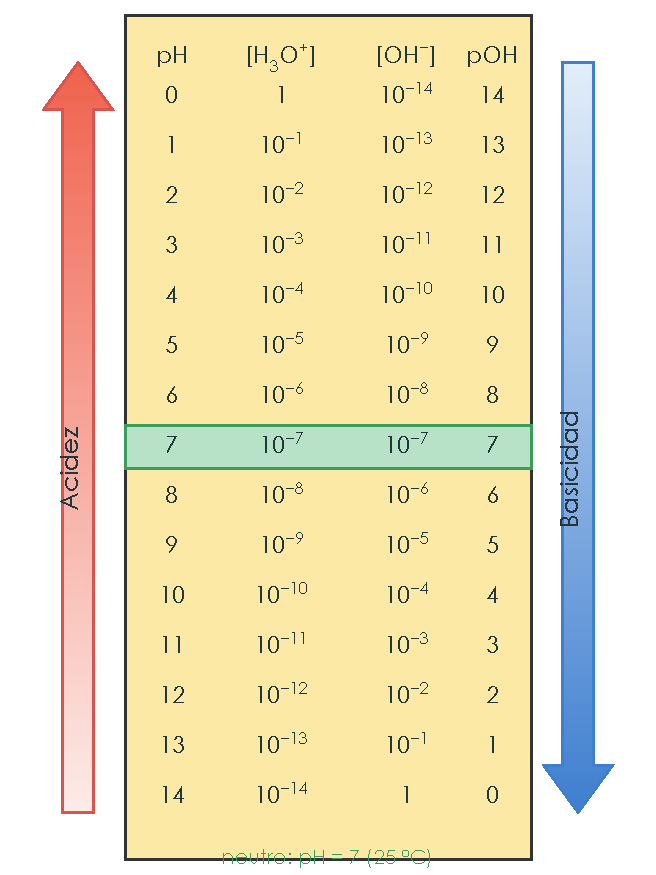
\includegraphics[width=0.5\linewidth]{FigurasSVG/UD7_Equilibrio_Acido_Base/pdf/UD7_02_escala_pH.pdf}
        \caption{Escala del pH y pOH junto con las concentraciones de \ch{H3O+} y \ch{OH-}}
        \label{fig:escala_ph}
    \end{figure}

    \section{Relación entre la constante de acidez de un ácido y la constante de basicidad de su base conjugada}

    La constante de acidez de un ácido (\Ka) la podemos relación con la constante de basicidad de su base conjugada (\Kb) a partir de la constante \Kw según la expresión:
    \begin{equation}
        \Ka \cdot \Kb = \Kw
    \end{equation}
    Si tomamos \( -\log \) en ambos términos y sabiendo que \( \Kw = \num{e-14} \) tendremos que:

    \begin{equation}
        \pKa + pKb = 14
    \end{equation}

    \section{Indicadores químicos}\label{sec:indicadores-quimicos}

    Para detectar las variaciones de pH normalmente se han utilizado \negrita{sustancias indicadoras} llamados \negrita{Indicadores} que a partir de ahora se abreviarán como \azuln{HIn} (forma ácida) o \rojon{\ch{In-}} (forma básica).

    Estos indicadores son ácidos o bases débiles que también experimentan un equilibrio pero tienen la peculiaridad de que tienen un color diferente en la forma ácida \negrita{\ch{HIn}} y en la forma básica \negrita{\negrita{\ch{In-}}} por lo que podemos escribir su correspondiente equilibrio y por tanto obtener su correspondiente constante de equilibrio que la representaremos como \(k_{\text{HIn}}\)

    \begin{equation*}
        \ch{!( "\textcolor{red}{Color\ A}" )(\color{red}HIn) + H2O <=> !( "\textcolor{blue}{Color\ B}" )(\color{blue}In-) + H3O+}
    \end{equation*}

    \begin{equation}
        k_{\text{HIn}} = \dfrac{\conc{In-}\ \conc{H3O+}}{\conc{HIn}}
    \end{equation}

    Al tratarse de ácidos y/o bases débiles ambas especies estarán presentes en el equilibrio.
    Para poder apreciar correctamente el cambio de color, la concentración de una de las especies debe ser al menos diez veces mayor que la concentración de la otra es decir:
    \begin{itemize}
        \item \negrita{Color ácido}: para ver el color de la forma ácida necesitaremos que al menos \(\conc{HIn} = 10\ \conc{In-}\).
        \item \negrita{Color básico}: para ver el color de la forma básica necesitaremos que al menos \(\conc{In-} = 10\ \conc{HIn}\).
    \end{itemize}

    Según lo visto, el cambio de color no se producirá a un valor fijo de pH si no que se hará en un intervalo de pH que vendrá determinada por la \(k_{\text{HIn}}\).

    Y ese intervalo será:

    \begin{equation}
        \text{pH} = \text{pk\subin{HIn}} \pm 1\label{eq:intervalo-indicar}
    \end{equation}

    A este intervalo de pH en el que se produce el cambio de color se le denomina \negrita{intervalo de viraje}


    Para llegar a la ecuación \eqref{eq:intervalo-indicar} debemos hacerlo en dos partes, estableciendo dos condiciones que se detallan a continuación:

    \begin{itemize}
        \item \textbf{Predomina el color de la forma ácida}, sería el \rojo{coloar A}. Si predomina el color de la forma ácida tendremos que \( \conc{HIn} = 10\ \conc{In-}  \).
        \begin{gather}
            K_{\ch{HIn}} = \dfrac{\conc{H3O+}\conc{In-}}{\conc{HIn}} \longrightarrow \conc{H3O+} = K_{\ch{HIn}} \cdot \dfrac{\conc{HIn}}{\conc{In-}} \notag \\[2mm]
            \text{tomamos } -\log \text{ en ambos términos}\notag \\[2mm]
            -\log{\conc{H3O+}} = -\log{\left( \dfrac{\conc{HIn}}{\conc{In-}} \right)} \notag \\[2mm]
            \pH = \text{pk\subin{HIn}}  -\log{\left( \dfrac{\conc{HIn}}{\conc{In-}} \right)} \notag \\[2mm]
             \pH = \text{pk\subin{HIn}}  -\log{\left( \dfrac{10\ \conc{In-}}{\conc{In-}} \right)} \notag \\[2mm]
            \pH = \text{pk\subin{HIn}}  -\log{10} \notag \\[2mm]
            \pH = \text{pk\subin{HIn}}  - 1 \label{eq:intervalo_ph_resta_1}
        \end{gather}
        \item \textbf{Predomina el color de la forma básica}, sería el \azul{coloar B}.
        Si predomina el color de la forma ácida tendremos que \( \conc{In-} = 10\ \conc{HIn}  \).
        \begin{gather}
            K_{\ch{HIn}} = \dfrac{\conc{H3O+}\conc{In-}}{\conc{HIn}} \longrightarrow \conc{H3O+} = K_{\ch{HIn}} \cdot \dfrac{\conc{HIn}}{\conc{In-}} \notag \\[2mm]
            \text{tomamos } -\log \text{ en ambos términos}\notag \\[2mm]
            -\log{\conc{H3O+}} = -\log{\left( \dfrac{\conc{HIn}}{\conc{In-}} \right)} \notag \\[2mm]
            \pH = \text{pk\subin{HIn}}  -\log{\left( \dfrac{\conc{HIn}}{\conc{In-}} \right)} \notag \\[2mm]
             \pH = \text{pk\subin{HIn}}  -\log{\left( \dfrac{\conc{HIn}}{10\ \conc{HIn}} \right)} \notag \\[2mm]
            \pH = \text{pk\subin{HIn}}  -\log{\dfrac{1}{10}} \notag \\[2mm]
            \pH = \text{pk\subin{HIn}}  + 1 \label{eq:intervalo_ph_suma_1}
        \end{gather}
    \end{itemize}

    Si combinamos las ecuaciones \eqref{eq:intervalo_ph_suma_1} y la ecuación \eqref{eq:intervalo_ph_resta_1} tendremos la ecuación \eqref{eq:intervalo-indicar}


%\begin{ejemplo}
%    Demostrar matemáticamente que el intervalo de viraje de un indicador estará en un intervalo de \(\text{pH} = \text{pk\subin{HIn}} \pm 1\)
%\end{ejemplo}

    \subsection{Elección del indicador}

    Debido a que el intervalo de viraje depende del propio indicador, no todos los indicadores son válidos para todas las disoluciones.


    El \negrita{indicador} apropiado será aquel que cambie de color en el intervalo de pH en el que se produzca la neutralización

    A continuación tenemos una tabla donde se indican los indicadores más comunes así como su intervalo de viraje y los colores de cada una de las formas.


    \begin{figure}[H]
        \centering
        % [FIGURA ORIGINAL] \includegraphics[scale=.7]{images/imagesUD7EquilibrioAcidoBase/UD7_Teoria/indicadores}
        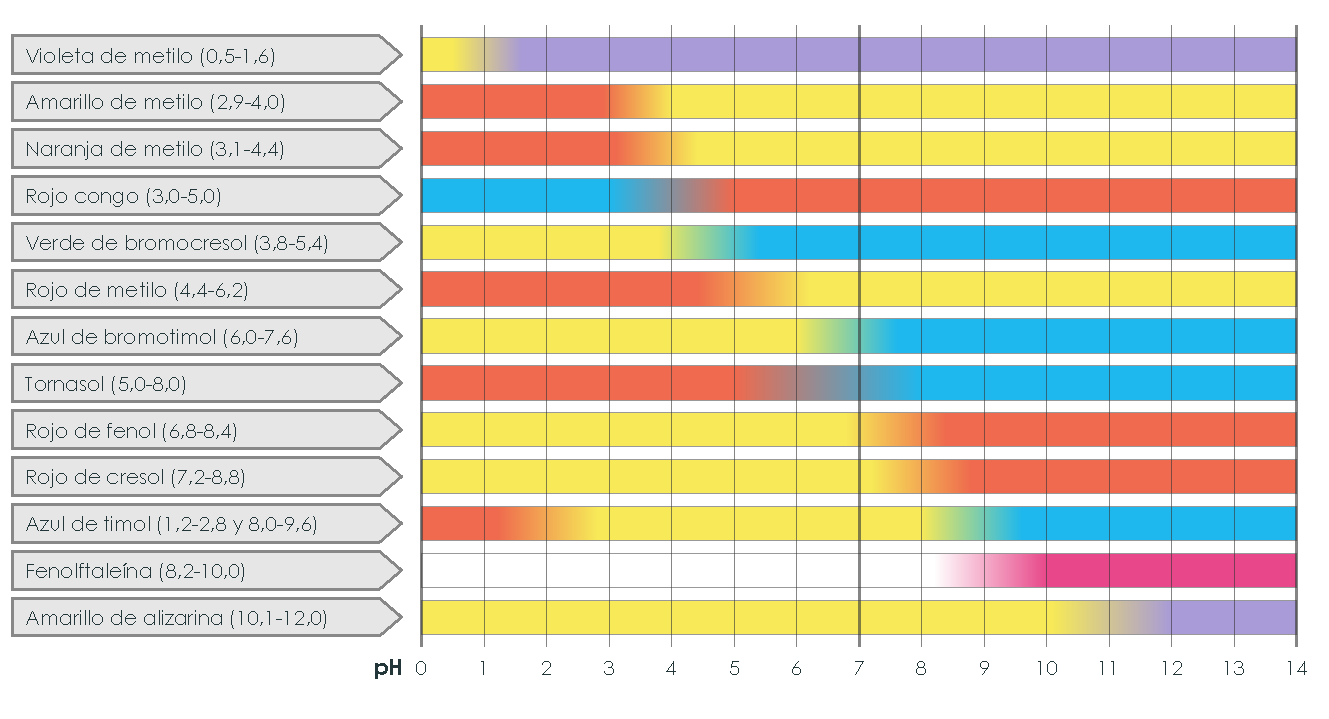
\includegraphics[width=0.95\linewidth]{FigurasSVG/UD7_Equilibrio_Acido_Base/pdf/UD7_03_indicadores.pdf}
        \caption{Colores de varios indicadores en función del pH}
        \label{fig:indicadores}
    \end{figure}

%\section{Ácidos y bases poliionizables}\label{sec:acidos-y-bases-poliionizables}
%
%Existen ácidos y bases que pueden experimentar sucesivas ionizaciones (tantas disociaciones como número de hidrógenos que tenga) y cada una de ellas tendrán su correspondiente equilibrio y por tanto su correspondiente constante.
%
%Consideremos primero el ejemplo del ácido sulfúrico \ch{H2SO4}.
%La disociación de este ácido sería:
%
%\begin{gather*}
%    \ch{H2SO4 + H2O -> HSO4- + H3O+}; \separ
%    \ch{HSO4- + H2O <=> SO4^{2-} + H3O+}; \quad k_{a2} = \num{e-2}\separ
%\end{gather*}
%
%La primera disociación del sulfúrico, se considera que se encuentra totalmente disociado y, por tanto, no tiene sentido dar un valor de \Ka{}.
%El segundo equilibrio, si se considera un ácido débil y, por tanto, se da su correspondiente constante de equilibrio.
%
%Para el caso del ácido carbónico, ahora ambas disociaciones se consideran débiles y, por tanto, se dan dos constantes de acidez.
%
%\begin{table}[H]
%    \centering
%    \begin{tblr}{c}
%        \( \ch{H2CO3 + H2O <=> HCO3- + H3O+}; \quad k_{a1} = \num{4.3e-7}\)\\
%        \(\ch{HCO3- + H2O <=> CO3^{2-} + H3O+}; \quad k_{a2} = \num{5.61e-11}\)\\
%    \hline
%    \( \ch{H2CO3 + 2 H2O <=> CO3^{2-} + 2 H3O+}; \quad k = k_{a1}\cdot k_{a2}\)
%    \end{tblr}
%\end{table}


    \section{Hidrólisis}\label{sec:hidrolisis}

    \begin{center}
        \begin{definicion}[width=0.9\textwidth]{Hidrólisis}
            La \negrita{hidrólisis} es cuando los iones de una sal reaccionan con el agua para generar de nuevo un ácido o una base
        \end{definicion}
    \end{center}


    Para su tratamiento, tenemos que disociar primer la sal en sus correspondientes iones y luego llevar a cabo la reacción entre cada ión con el agua.

    \subsection{Sal de ácido fuerte y base fuerte}\label{subsec:sal-de-acido-fuerte-y-base-fuerte}

    Consideremos un ácido fuerte como \ch{HCl} y una base fuerte \ch{NaOH}.
    Ambos reaccionan según la siguiente reacción produciendo \ch{NaCl} y agua:
    \begin{equation*}
        \ch{HCl + NaOH -> NaCl + H2O}
    \end{equation*}
    La sal formada, por tanto, será el \ch{NaCl}, si disociamos esta sal tendremos:
    \begin{equation*}
        \ch{NaCl -> Na+ + Cl-}
    \end{equation*}

    Como el \ch{Na+} es el ácido conjugado de una base fuerte, entonces será un ácido débil y \negrita{no} reaccionará con el agua.

    Como el \ch{Cl-} es base conjugado de un ácido fuerte, entonces será una base débil y \negrita{no} reaccionará con el agua.

    Podemos resumir entonces, que los ácidos y bases conjugadas procedentes de ácidos y bases fuertes no reaccionarán con el agua, es decir no se producirá hidrólisis de los mismos.

    \caja{En este tipo de caso tendremos una disolución con \(\pH=7\) es decir una disolución \negrita{neutra}.}

    \subsection{Sal de ácido débil y base fuerte}\label{subsec:sal-de-acido-debil-y-base-fuerte}

    Consideremos ahora la reacción entre un ácido débil por ejemplo el ácido acético, que lo podemos esquematizar como \ch{HAc} y el hidróxido de potasio \ch{KOH} que es una base fuerte.
    La reacción que tendrá lugar será:
    \begin{equation*}
        \ch{HAc + KOH -> AcK + H2O}
    \end{equation*}

    Ahora, el acetato de potasio formado, lo podemos disociar en:

    \begin{equation*}
        \ch{AcK -> Ac- + K+}
    \end{equation*}

    El ácido conjugado \ch{K^+} al proceder de una base fuerte, no reaccionará con el agua puesto que es un ácido débil.
    Ahora, la base conjugada acetato \ch{Ac-} es una base fuerte, puesto que procede de un ácido débil y por tanto si reaccionará con el agua según la reacción:

    \begin{equation*}
        \ch{ Ac- + H2O <=> HAc + OH-}
    \end{equation*}

    Como vemos, se vuelve a formar el ácido conjugado del que procede y también iones hidroxilo.
    La constante de este equilibrio y, en consecuencia, la constante de hidrólisis \Kh{} será.
    \begin{equation}
        \Kh = \dfrac{\conc{HAc}\ \conc{OH-}}{\conc{Ac-}} \label{eq:cte_hidrolisis_base}
    \end{equation}

    \caja{En este tipo de caso tendremos una disolución con \(\text{pH}>7\) es decir una disolución \negrita{básica}.}

    Esta constante de hidrólisis \Kh la podemos relacionar con la correspondiente constante de acidez del ácido conjugado \ch{HAc} y con el producto iónico del agua sabiendo que:
    \begin{gather*}
        \ch{HAc + H2O <=> Ac- + H3O+}\separ
        \Ka = \dfrac{\conc{Ac-}\ \conc{H3O+}}{\conc{HAc}}
    \end{gather*}

    Si la expresión \eqref{eq:cte_hidrolisis_base} la multiplicamos y dividimos por la concentración de iones oxonio \ch{H3O+} tendremos que:

    \begin{equation*}
        \Kh = \dfrac{{\color{blue}\conc{HAc}}\ {\color{red}\conc{OH-}}}{{\color{blue}\conc{Ac-}}}\dfrac{{\color{red}\conc{H3O+}}}{{\color{blue}\conc{H3O+}}}
    \end{equation*}
    como podemos ver:
    \begin{equation*}
        \color{blue} \dfrac{1}{\Ka} = \dfrac{\conc{HAc}}{\conc{Ac-}\ \conc{H3O+}}
    \end{equation*}
    y que:
    \begin{equation*}
        \color{red} \Kh = \conc{H3O+}\ \conc{OH-}
    \end{equation*}
    Por lo tanto, podemos decir que:
    \begin{equation*}
        \Kh = \dfrac{{\color{red}\Kw}}{{\color{blue}\Ka}}
    \end{equation*}
    
    Esta \Kh hace referencia en este caso a la constante de equilibrio de la especie \ch{Ac-} por lo que la podemos escribir como K\textsubscript{\ch{Ac-}} y como el acetato es una base también la podemos escribir como \Kb

    \subsection{Sal de ácido fuerte y base débil}\label{subsec:sal-de-acido-fuerte-y-base-debil}

    Consideremos ahora el caso entre la reacción entre un ácido fuerte \ch{HCl} y una base débil como el amoniaco \ch{NH3}.
    Ambas especies darán lugar a la siguiente reacción:
    \begin{equation*}
        \ch{HCl + NH3 -> NH4Cl + H2O}
    \end{equation*}

    Ahora el cloruro de amonio formado lo podemos disociar en:

    \begin{equation*}
        \ch{NH4Cl -> NH4+ + Cl-}
    \end{equation*}

    El ión \ch{Cl-} es una base débil, ya que proviene de un ácido fuerte y, por tanto, no reaccionará con el agua.
    El \ch{NH4+} es un ácido fuerte, ya que proviene de una base débil y, por tanto, si reaccionará con el agua según la reacción:

    \begin{equation*}
        \ch{NH4+ + H2O  <=> NH3 + H3O+}
    \end{equation*}

    En este caso, la constante de hidrólisis será:
    \begin{equation}
        \Kh = \dfrac{\conc{NH3}\ \conc{H3O+}}{\conc{NH4+}} \label{eq:cte_hidrolisis_acido}
    \end{equation}

    \caja{En este tipo de casos tendremos una disolución de \(\text{pH}<7\) es decir una disolución \negrita{ácida}.}


    De manera análoga al caso anterior, podemos relacionar la constante de hidrólisis con la constante de basicidad de la base formada en la hidrólisis, siendo en este caso el \ch{NH3}.

    Si la expresión \eqref{eq:cte_hidrolisis_acido} la multiplicamos y dividimos por la concentración de iones oxonio \ch{OH-} tendremos que:

    \begin{equation*}
        \Kh = \dfrac{{\color{blue}\conc{NH3}}\ {\color{red}\conc{H3O+}}}{{\color{blue}\conc{NH4+}}}\dfrac{{\color{red}\conc{OH-}}}{{\color{blue}\conc{OH-}}}
    \end{equation*}
    como podemos ver:
    \begin{equation*}
        \color{blue} \dfrac{1}{k_a} = \dfrac{\conc{NH3}}{\conc{NH4+}\ \conc{OH-}}
    \end{equation*}
    y que:

    \begin{equation*}
        \color{red} \Kh = \conc{H3O+}\ \conc{OH-}
    \end{equation*}

    Por lo tanto, podemos decir que:

    \begin{equation}
        \Kh = \dfrac{{\color{red}\Kw}}{{\color{blue}\Kb}}
    \end{equation}

    Esta \Kh hace referencia en este caso a la constante de equilibrio de la especie \ch{NH4+} por lo que la podemos escribir como K\textsubscript{\ch{NH4+}} y como el acetato es un ácido también la podemos escribir como \Ka

    \subsection{Sal de ácido débil y base débil}\label{subsec:sal-de-acido-debil-y-base-debil}

    Imaginemos ahora la reacción entre ácido acético \ch{HAc} y \ch{NH3}.

    \begin{equation*}
        \ch{HAc + NH3 -> AcNH4}
    \end{equation*}

    La sal formada \ch{AcNH4} se disociará según:
    \begin{equation*}
        \ch{AcNH4 -> Ac- + NH4+}
    \end{equation*}

    En este caso, ambas especies reaccionarán con el agua al proceder de ácidos y bases débiles, teniendo entonces que:
    \begin{equation}
        \begin{aligned}
            \ch{NH4+ + H2O & <=> NH3 + H3O+}\separ
            \ch{ Ac- + H2O & <=> HAc + OH-}\separ
            \midrule
            \ch{Nh4+ + Ac- +} \cancelred{\ch{2 H2O}} & <=> \ch{NH3 + HAc +} \cancelred{\ch{OH- + H3O+}}
        \end{aligned}
    \end{equation}
    En este caso, la constante de hidrólisis quedaría como:
    \begin{equation}
        \Kh = \dfrac{\conc{NH3}\ \conc{HAc}}{\conc{NH4+}\ \conc{Ac-}} \label{eq:cte_hidrolisis_acido_base}
    \end{equation}
    Si ahora la expresión \eqref{eq:cte_hidrolisis_acido_base} la multiplicamos y dividimos por \conc{H3O+} \conc{OH-} tendremos que:

    \begin{equation*}
        \Kh = \dfrac{{\color{red}\Kw}}{{\color{blue}\Ka \cdot \Kb}}
    \end{equation*}
    \caja{En este caso, el valor del \pH{} dependerá de la fortaleza de cada especie, si \(\Ka>\Kb\) entonces la disolución será básica y si \( \Ka < \Kb \) entonces la disolución será ácida.}


    \section{Disoluciones tampón}\label{sec:disoluciones-tampon}

    Las disoluciones tampón, también se llaman disoluciones \negrita{buffers}, \negrita{reguladoras} o \negrita{amortiguadoras} y son disoluciones que permiten mantener sin variar el pH de la disolución tras añadir un ácido o una base.

    ¿Cómo son capaces de hacerlo?
    Estas disoluciones son capaces de absorber un exceso de iones hidroxilo o un exceso de iones oxonio.

    Estas disoluciones pueden ser de dos tipos:
    \begin{enumerate}[label=\numberballmDarkTeal]
        \item \negsubro{Ácido débil y su sal}.
        Por ejemplo la mezcla entre \ch{CH3COOH + CH3COONa}.

        Cuando tenemos estas mezclas tendremos, por tanto, el siguiente equilibrio:

        \begin{equation*}
            \ch{CH3COOH + H2O <=> CH3COO- + H3O+}
        \end{equation*}

        Si escribimos la ecuación de la constante de equilibrio del \ch{CH3COOH}, despejamos la concentración de oxonio y luego tomamos \( -\log  \) en ambos términos tendremos una expresión que nos permite calcular el \pH{} de esa disolución reguladora:

%        Para calcular el pH de esta disolución reguladora se realiza según la expresión:
%        \begin{equation*}
%            \pH = \pKa + \log\dfrac{\conc{Sal}}{\conc{Ácido}}
%        \end{equation*}

%        En este caso tendríamos que:

        \begin{equation*}
            \pH = \pKa + \log\dfrac{\conc{CH3COO-}}{\conc{CH3COOH}}
        \end{equation*}

        En esta expresión, las cantidades disociadas se desprecian, puesto que son muy pequeñas comparadas con las cantidades de sal y de ácido que se añaden, simplificando así los cálculos.

        Al añadir una base, los iones hidroxilo reaccionan con el acético neutralizándose.
        De esta manera se evita que la disolución se vuelva básica.
        \begin{equation*}
            \ch{CH3COOH + OH- -> CH3COO- + H2O}
        \end{equation*}
        Cuando se añade un ácido, los iones oxonio se retiran de la disolución combinándose con \ch{CH3COO-} evitando así que la disolución se vuelva ácida.
        \begin{equation*}
            \ch{CH3COO- + H3O+ -> CH3COOH + H2O}
        \end{equation*}
        \item \negsubro{Base débil y su sal}.
        Por ejemplo la mezcla entre \ch{NH3 + NH4Cl}.

        Cuando tenemos estas mezclas tendremos, por tanto, el siguiente equilibrio:

        \begin{equation*}
            \ch{NH3 + H2O <=> NH4 + OH-}
        \end{equation*}

        Para calcular el pH de esta disolución reguladora se calcula primero el \pOH{} según la expresión:
        \begin{equation*}
            \pOH = \pKb + \log\dfrac{\conc{Sal}}{\conc{Base}}
        \end{equation*}

        En este caso tendríamos que:

        \begin{equation*}
            \pOH = \pKb + \log\dfrac{\conc{NH4+}}{\conc{NH3}}
        \end{equation*}

        Una vez calculado el \pOH{} calculamos el \pH{} según:

        \begin{equation*}
            \pH + \pOH = 14
        \end{equation*}

        Al añadir una base, los iones hidroxilo reaccionan con el amonio neutralizándose evitando así que la disolución se vuelva básica.
        \begin{equation*}
            \ch{NH4+ + OH- -> NH3 + H2O}
        \end{equation*}
        Cuando se añade un ácido, los iones oxonio se retiran de la disolución combinándose con \ch{NH3} evitando así que la disolución se vuelva ácida.
        \begin{equation*}
            \ch{NH3 + H3O+ -> NH4+ + H2O}
        \end{equation*}
    \end{enumerate}

% \begin{problemas}
%     \problema{. 86}. 
%     % Si se tienen \volumen[ml]{100} de una disolución de ácido etanoico \concentracion[m]{0.2}, ¿con cuál de las siguientes disoluciones lo mezclarías para formar la mejor disolución tampón posible?
%     % \begin{enumerate}[label=\letraminuscula]
%     %     \item \volumen[ml]{100} de disolución de \ch{CH3COONa} a \concentracion[m]{0.1}.
%     %     \item \volumen[ml]{100} de disolución de \ch{NaOH} a \concentracion[m]{0.1}.
%     %     \item \volumen[ml]{200} de disolución de \ch{CH3COONa} a \concentracion[m]{0.1}.
%     %     \item \volumen[ml]{100} de disolución de \ch{NaOH} a \concentracion[m]{0.2}.
%     % \end{enumerate}

%     \problema{. 96} 

%     \problema{. 105}. ¿Cuál es la variación en el \pH característico de una disolución reguladora que es \concentracion[m]{0.1} en ácido acético y 0,1 M en acetato de sodio, cuando a 1 L de la misma se le añaden 0,005 moles de  \ch{HCl}? Se desprecia la variación de volumen. 
% \end{problemas}


    \section{Valoraciones ácido-base}\label{sec:valoraciones-acido-base}

    Para determinar la concentración de una disolución de un ácido o una base se recurre a neutralizarla con otra disolución (base o ácido respectivamente) cuya concentración es conocida obteniéndose la concentración de la disolución desconocida a partir de las cantidades gastadas de una y de otra.

    A este procedimiento se le denomina \negrita{volumetría ácido-base}.

    Cuando ha reaccionado todo el ácido con toda la base, decimos que hemos llegado al \negrita{punto de equivalencia}

    \subsection{Procedimiento operativo}\label{subsec:procedimiento-operativo}

    Un procedimiento general sería:
    \begin{itemize}
        \item Medir con exactitud un volumen de la disolución de concentración desconocida con una pipeta y ponerlo en un matraz Erlenmeyer.
        \item Verter en una bureta, la disolución de concentración conocida.
        \item Añadir 1 ó 2 gotas de un indicador químico a la disolución de concentración desconocida que tenemos en el matraz Erlenmeyer.
        \item Añadir gota a gota desde la bureta hasta el matraz Erlenmeyer removiendo la disolución desconocida durante la adición.
        Se recomienda poner un papel blanco debajo del Erlenmeyer para visualizar mejor el cambio de color.
        \item Cuando se produce el cambio de color del indicador, leer el volumen gastado en la bureta.
    \end{itemize}

    \subsection{Cálculos estequiométricos}\label{subsec:calculos-estequiometricos}

    Al llegar a la neutralización, los moles de \ch{H3O+} y los moles de \ch{OH-} que han reaccionado tienen que ser los mismos.
    Podemos realizar los cálculos de varias manera:

    \negsubro{Método 1}:

    \begin{enumerate}[label=\numberballmDarkTeal]
        \item Escribiendo la reacción ajustada que tiene lugar y llevar a cabo los cálculos estequiométricos.
        \item Si nos dan los datos de concentración molar y volumen podremos, escribir la reacción ajustada que tiene lugar y aplicar la fórmula:

        \begin{equation}
            n_{\text{base}}\cdot M_{\text{ácido}}\cdot V_{\text{ácido}} = n_{\text{ácido}}\cdot M_{\text{Base}}\cdot V_{\text{Base}}\label{eq:valoracion-acido-base-ecuacion}
        \end{equation}

        Siendo \(n_{\text{base}}\) el coeficiente estequiométrico de la base, \(n_{\text{ácido}}\) el coeficiente estequiométrico del ácido y \(M_{\text{ácido}}\) y \(M_{\text{ácido}}\)
    \end{enumerate}

    \negsubro{Método 2}:

    \begin{enumerate}[label=\numberballmDarkTeal]
        \item Utilizando la Normalidad y la ecuación:

        \begin{equation*}
            \text{nº eq-g ácido} =  \text{nº eq-g base}
        \end{equation*}

        Esta última expresión lo podemos poner en función de la normalidad y del volumen según:

        \begin{equation*}
            N_{\text{ácido}}\cdot V_{\text{ácido}} =  N_{\text{Base}}\cdot V_{\text{Base}}
        \end{equation*}

        Si lo que queremos es una expresión, en la que se tenga la molaridad, sabiendo que \(N = M \cdot \text{valencia}\) tendremos que:

        \begin{equation}
            \text{valencia\subin{ácido}}\cdot M_{\text{ácido}}\cdot V_{\text{ácido}} = \text{valencia\subin{base}}\cdot M_{\text{Base}}\cdot V_{\text{Base}}
        \end{equation}

    \end{enumerate}

    \negsubro{RECORDATORIO}:

    \begin{equation*}
        N = \dfrac{n^\text{º}\ eq-g}{\text{V(L)}}; \qquad n^\text{º}\ eq-g = \dfrac{m(g)}{P_{eq}} \qquad P_{eq} = \dfrac{M_w}{Valencia}
    \end{equation*}

    Siendo \(n^\text{º}\ eq-g\) el número de equivalentes gramo de dicha especie, \(P_{eq}\) es el peso equivalente, \(M_w\) es la masa molecular.

    Para calcular la valencia en los equilibrios ácido-base, podemos seguir la siguiente regla.

    \begin{itemize}
        \item \negrita{Ácidos}: Será el número de hidrógenos que se transfiera en la reacción.
        \item \negrita{Bases}: Será el número de iones hidroxilo que tenga dicha especie.
        En el caso de no tener grupos hidroxilo como es el caso del amoniaco, será el número de hidrones que pueda aceptar.
    \end{itemize}

    \subsection{Curvas de valoración}\label{subsec:curvas-de-valoracion}

    Una curva de valoración es la representación del pH frente al volumen de agente valorante.
    Dependiendo de la naturaleza de cada reactivo, la curva de valoración será diferente.
    \begin{enumerate}[label=\numberballmDarkTeal]
        \item \negsubro{Ácido débil - Base fuerte}: el punto de equivalencia se encuentra en un intervalo no muy grande en un pH ligeramente básico.
        Siendo su gráfica:

        \begin{figure}[H]
            \centering
            % [FIGURA ORIGINAL] \includegraphics[scale=0.7]{images/imagesUD7EquilibrioAcidoBase/UD7_Teoria/acido_debil_base_fuerte}\label{fig:acidodebil-base-fuerte}
            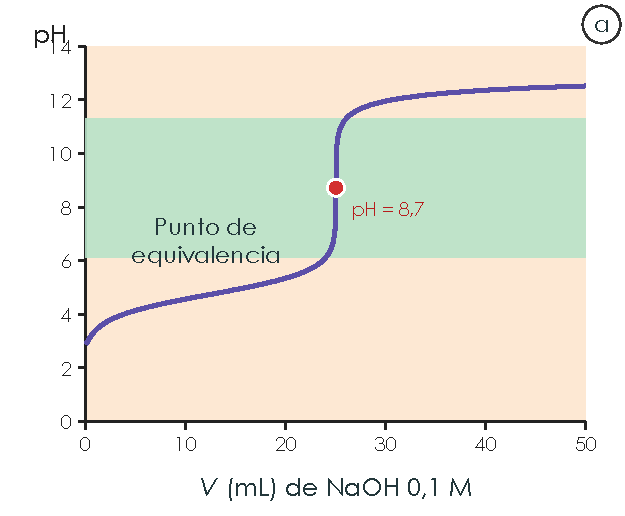
\includegraphics[width=0.55\linewidth]{FigurasSVG/UD7_Equilibrio_Acido_Base/pdf/UD7_04_valoracion_acido_debil_base_fuerte.pdf}\label{fig:acidodebil-base-fuerte}
        \end{figure}

        \item \negsubro{Base débil - Ácido fuerte}: muy parecido al caso anterior, pero en este caso el intervalo de viraje en el pH será ligeramente ácido.

        \begin{figure}[H]
            \centering
            % [FIGURA ORIGINAL] \includegraphics[scale=0.7]{images/imagesUD7EquilibrioAcidoBase/UD7_Teoria/base_debel_acido_fuerte}\label{fig:basedebil-acido-fuerte}
            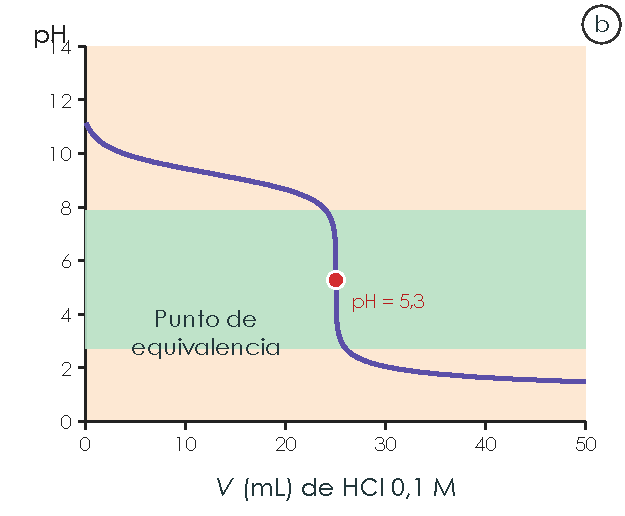
\includegraphics[width=0.55\linewidth]{FigurasSVG/UD7_Equilibrio_Acido_Base/pdf/UD7_05_valoracion_base_debil_acido_fuerte.pdf}\label{fig:basedebil-acido-fuerte}
        \end{figure}

        \item \negsubro{Ácido fuerte - Base fuerte}: el intervalo del pH en el punto de equivalencia es muy grande lo que permite usar muchos indicadores.

        \begin{figure}[H]
            \centering
            % [FIGURA ORIGINAL] \includegraphics[scale=0.7]{images/imagesUD7EquilibrioAcidoBase/UD7_Teoria/acido_fuerte_base_fuerte}\label{fig:acidofuerte-base-fuerte}
            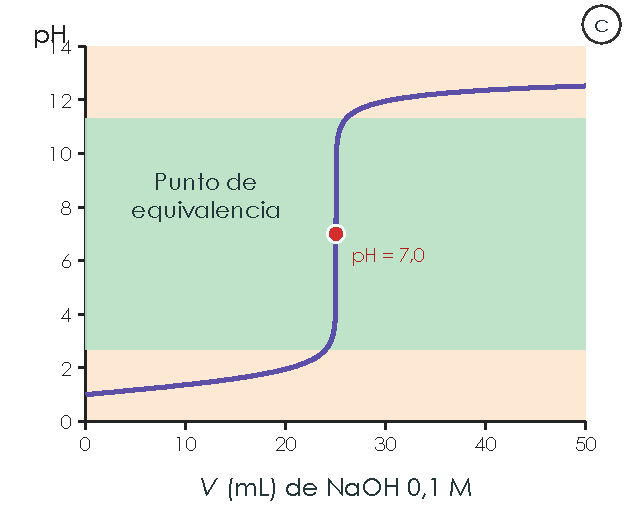
\includegraphics[width=0.55\linewidth]{FigurasSVG/UD7_Equilibrio_Acido_Base/pdf/UD7_06_valoracion_acido_fuerte_base_fuerte.pdf}\label{fig:acidofuerte-base-fuerte}
        \end{figure}

        \item \negsubro{Ácido débil - Base débil}: el intervalo en el pH en el punto de equivalencia es muy estrecho lo que resulta muy difícil su determinación.

        \begin{figure}[H]
            \centering
            % [FIGURA ORIGINAL] \includegraphics[scale=.7]{images/imagesUD7EquilibrioAcidoBase/UD7_Teoria/acido_debil_base_debil}\label{fig:acido-debil-base-debil}
            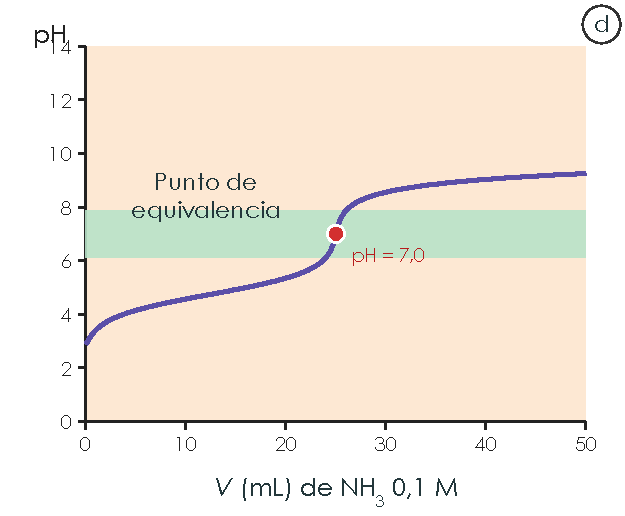
\includegraphics[width=0.55\linewidth]{FigurasSVG/UD7_Equilibrio_Acido_Base/pdf/UD7_07_valoracion_acido_debil_base_debil.pdf}\label{fig:acido-debil-base-debil}
        \end{figure}

    \end{enumerate}


